% Drawing 156-8/01-1 -- folder 156-8, batch 01, archive page 3 (PDF page 4).
% Transcription: en marge de Magor~1', une petite boucle d'un point $x$ à $Y$.
% Kind: marginal sketch (loop). Method 2 (schematic redraw from the facsimile). Status: ok.
% Notes: A small loop drawn from the point x out to Y and back, with an arrow; the struck words and the text around it (« NB ... X < Y ») belong to the transcription.
% Coordinates: 1 unit = 1 mm = 1/100 of the crop width (bbox in page fractions: [0.66, 0.36, 0.93, 0.5]).
% Redrawn by Claude (claude-opus-5-5), issue #73 pilot, 2026-11-07; not checked by a human; not compiled (no TeX in the session).
% Rights: reproduces part of the work -- behind RENDER_TRANSCRIPTS, never published by itself.
\documentclass[tikz,border=3pt]{standalone}
\usepackage{amsmath,amssymb}
\usetikzlibrary{patterns,arrows.meta}
\tikzset{pencil/.style={black!45}, struck/.style={black!35}, mark/.style={circle,draw,inner sep=1.3pt}, pt/.style={circle,fill,inner sep=0.9pt}, opt/.style={circle,draw,fill=white,inner sep=1.1pt}}
\begin{document}
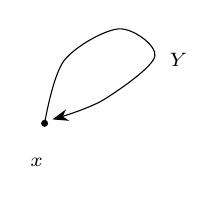
\begin{tikzpicture}[x=1mm,y=1mm,line cap=round,line join=round,font=\scriptsize]
\node[pt] at (44.5,-57) {};
\draw[-{Stealth[length=2mm]}] plot[smooth, tension=0.55] coordinates {(44.5,-57) (47,-49) (54,-45) (58.5,-48.5) (52,-54) (45.5,-56.5)};
\node[inner sep=1pt] at (43.5,-62) {\scriptsize $x$};
\node[inner sep=1pt] at (61.5,-49) {\scriptsize $Y$};
\end{tikzpicture}
\end{document}
